\documentclass{beamer}
\usefonttheme{serif}
\usepackage{graphicx}
\usepackage{xcolor}
\usepackage{colortbl}
\usepackage{multirow,tabularx}
\usepackage{tikz}
\usepackage{hyperref}
\hypersetup{
    colorlinks=true,
    linkcolor=blue,
    filecolor=blue,
    urlcolor=blue,
    pdftitle={Anomaly Detection: An Introduction},
    pdfpagemode=FullScreen,
    }
\usepackage{physics}
\usepackage{siunitx}
\usepackage{amsthm}
\usepackage{amsmath}

% Definition block formatting
\setbeamertemplate{theorems}[numbered]
\setbeamercolor{block title}{use=structure,fg=white,bg=structure.fg!75!black}
\setbeamercolor{block body}{parent=normal text,use=block title,bg=block title.bg!10!bg}

% Package for figure captions
\usepackage[font=small,skip=2pt]{caption}
\setlength{\belowcaptionskip}{-10pt}

% Define blue color
\definecolor{purple}{rgb}{0.3, 0.0, 0.557}
\definecolor{blue}{rgb}{0.0234375, 0.11328125, 0.609375}

\usepackage{multicol}
\usepackage{wrapfig}

% Use blue theme for the presentation
\setbeamercolor{frametitle}{fg=blue}
\setbeamercolor{title}{fg=blue}
\setbeamercolor{structure}{fg=blue}

\title{\textcolor{blue}{Anomaly Detection: An Introduction}}
\subtitle{\textcolor{blue}{Wigner Summer Camp \\ Data and Compute Intensive Sciences Research Group}}
\author{\textcolor{blue}{Balázs, Paszkál, Vince, Levente, Bence, Antal \\ Éva, Hajni}}

\date{\textcolor{blue}{6--10 July 2026}}

% Redefine footline to show only the slide number on the bottom left in blue
\setbeamertemplate{footline}
{
  \leavevmode%
  \hbox{%
  \begin{beamercolorbox}[wd=.1\paperwidth,ht=2.25ex,dp=1ex,left]{page number in head/foot}%
    \hspace{1em} \textcolor{blue}{\insertframenumber}%
  \end{beamercolorbox}}%
  \vskip0pt%
}

\begin{document}

\begin{frame}
  \titlepage
  \begin{columns}
    \centering
    \column{0.3\textwidth}
    \column{0.3\textwidth}
    \centering
    
\includegraphics[width=0.8\textwidth]{../img/logo.png}
    \column{0.3\textwidth}
  \end{columns}
\end{frame}

\begin{frame}{Contents}
    \tableofcontents
\end{frame}

% ==============================================================
\section{Why Anomaly Detection?}

\begin{frame}{Why Anomaly Detection Matters}
  \begin{itemize}
    \item Most data is \emph{normal}; the rare exceptions are often what matter most.
    \item An \textbf{anomaly} can signal a fault, a fraud, a fault-line tremor, or a new discovery.
    \item Real-world examples appear everywhere:
    \begin{itemize}
      \item A machine vibrating differently just before it breaks.
      \item An unusual transaction hinting at a stolen credit card.
      \item An abnormal heartbeat in a patient's ECG.
      \item A faint, unexpected signal in a physics experiment.
    \end{itemize}
    \item These events are \textbf{rare}, so we cannot rely on labelled examples of every failure.
    \item We must instead learn what \emph{normal} looks like, and flag whatever deviates from it.
  \end{itemize}
\end{frame}

% ==============================================================
\section{From Data to Anomalies}

\begin{frame}{Time Series}
  \begin{itemize}
    \item A \textbf{time series} is a quantity measured as a function of time.
    \item It is the raw data we work with throughout this camp.
    \item Our goal is to find the interesting moments hidden inside it.
  \end{itemize}
  \begin{center}
    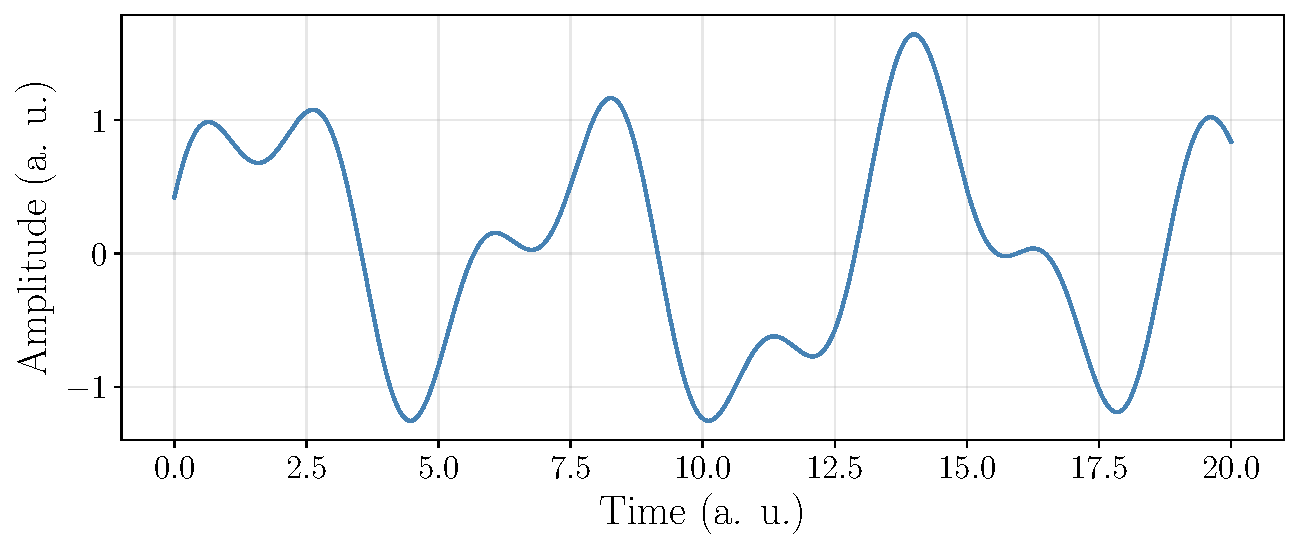
\includegraphics[width=0.78\textwidth]{../img/intro_time_series.pdf}
  \end{center}
\end{frame}

\begin{frame}{Peaks}
  \begin{itemize}
    \item A \textbf{peak} is a sample that is larger than its neighbours.
    \item Peaks often mark the events we care about.
    \item Detecting them reliably is a core building block of our pipeline.
  \end{itemize}
  \begin{center}
    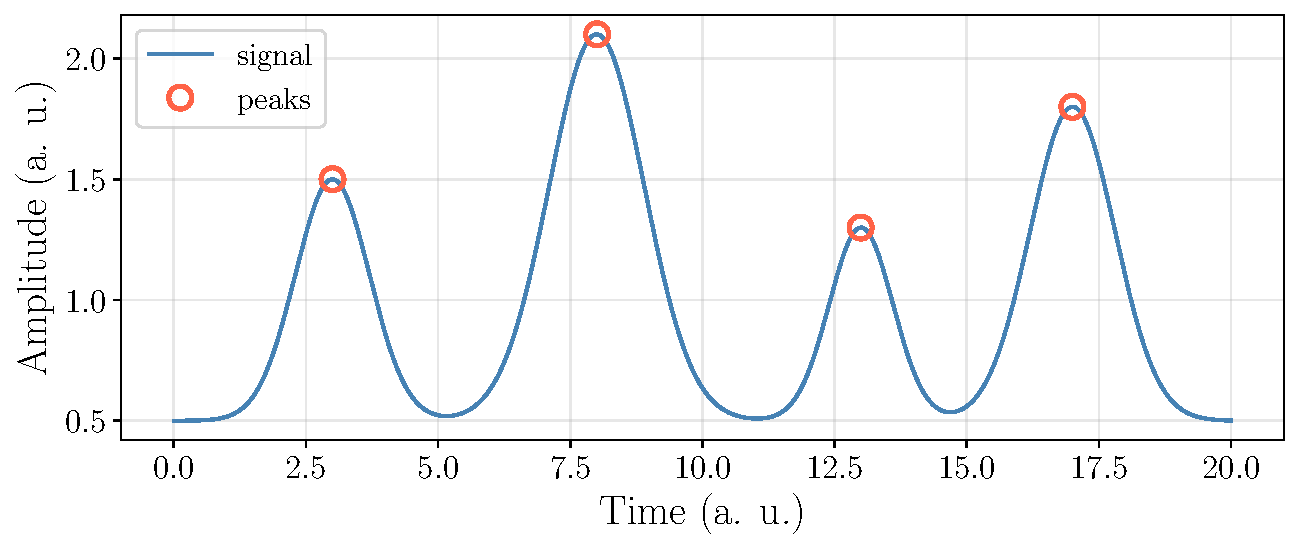
\includegraphics[width=0.78\textwidth]{../img/intro_peaks.pdf}
  \end{center}
\end{frame}

\begin{frame}{Anomalies}
  \begin{itemize}
    \item An \textbf{anomaly} is a sample that breaks the normal behaviour of the signal.
    \item Here the normal behaviour is a noisy sine, and the spikes are the anomalies.
    \item Finding these rare, unexpected events is the heart of anomaly detection.
  \end{itemize}
  \begin{center}
    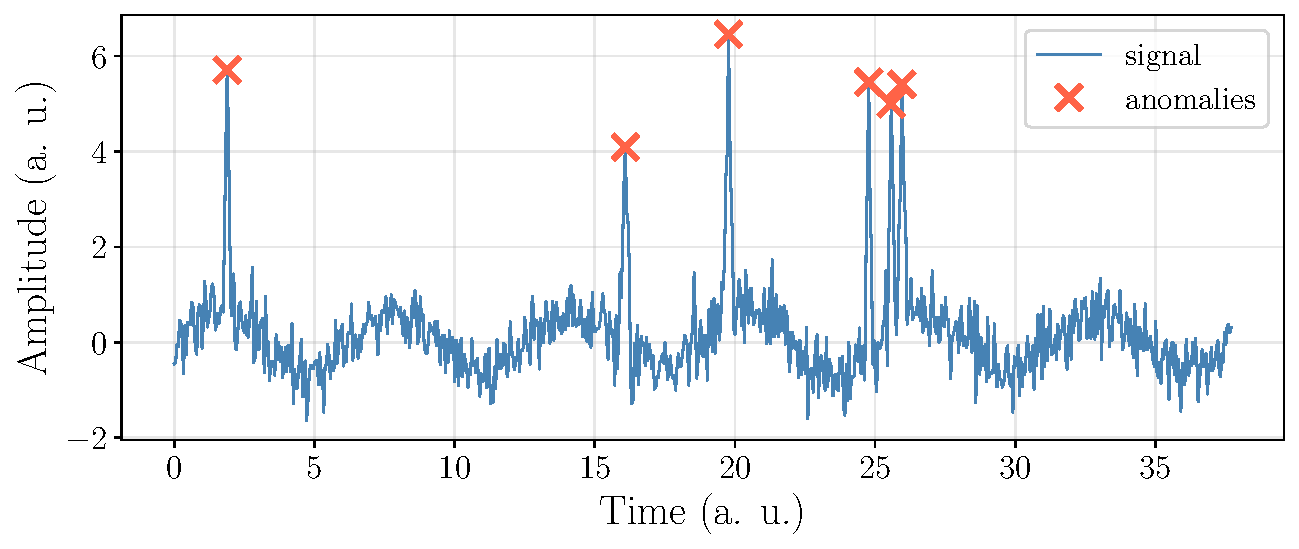
\includegraphics[width=0.78\textwidth]{../img/intro_anomaly.pdf}
  \end{center}
\end{frame}

% ==============================================================
\section{Detecting Anomalies}

\begin{frame}{Transforming the Data with \texttt{altx}}
  \begin{itemize}
    \item Anomalies can be hard to spot directly in a noisy signal.
    \item The \textbf{\texttt{altx}} method learns the normal dynamics and turns the signal into an \emph{anomaly score}.
    \item This score stays small for normal data and rises sharply at the anomalies.
  \end{itemize}
  \begin{center}
    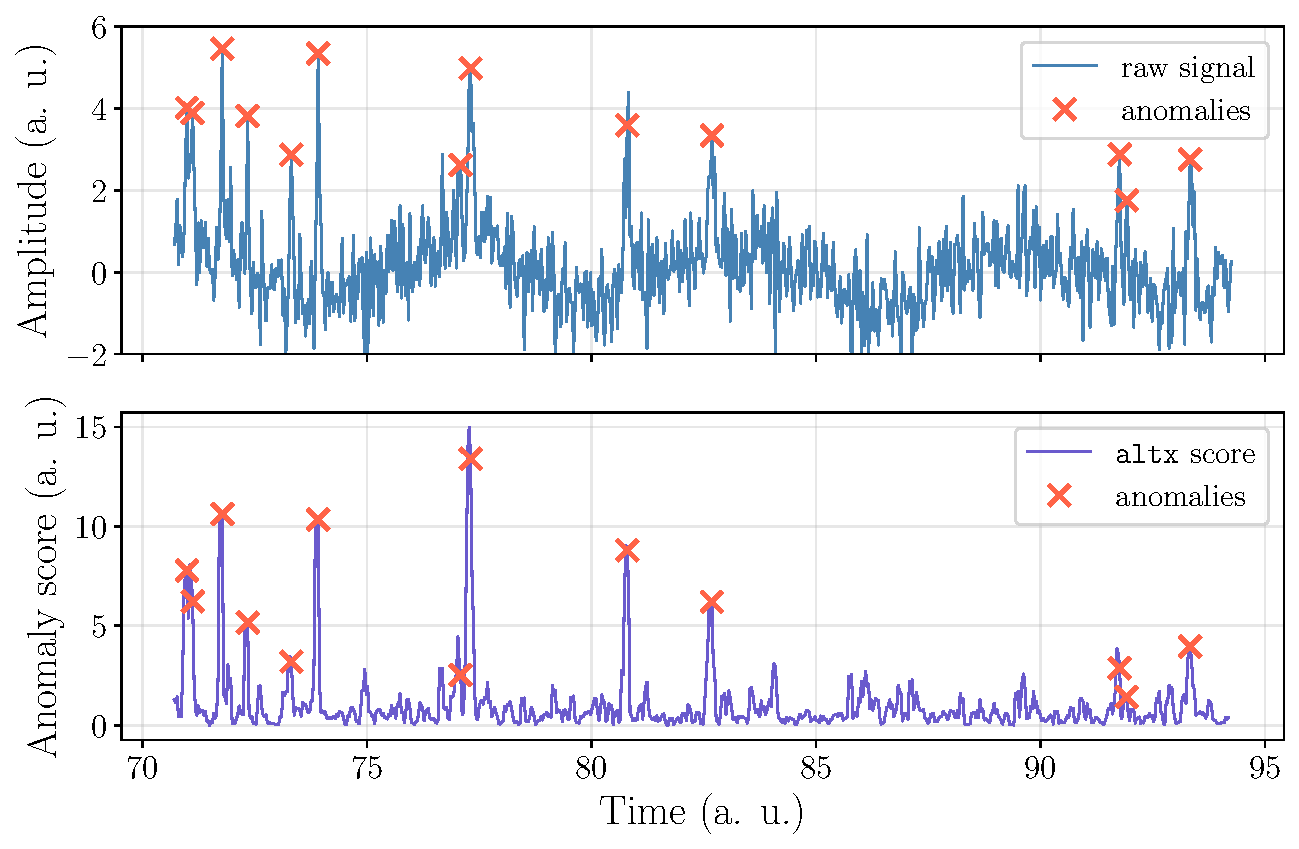
\includegraphics[width=0.66\textwidth]{../img/intro_altx_transformed.pdf}
  \end{center}
\end{frame}

\begin{frame}{Detecting the Anomalies}
  \begin{itemize}
    \item On the transformed score, the anomalies become clear peaks.
    \item We then run peak detection to locate them automatically.
    \item The detected peaks match the true anomalies closely.
  \end{itemize}
  \begin{center}
    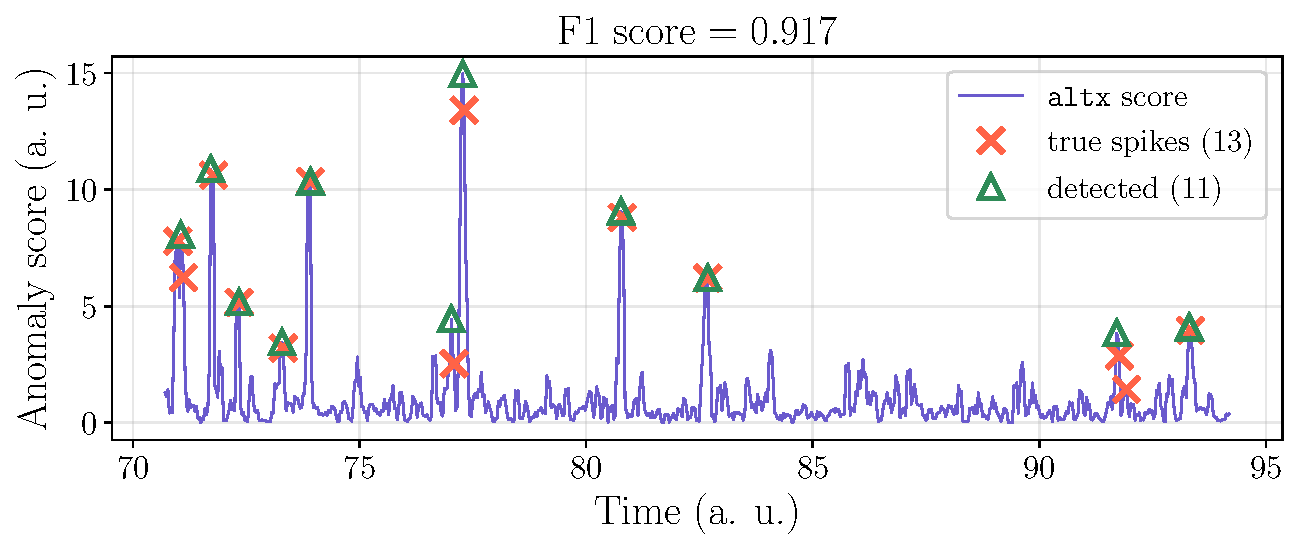
\includegraphics[width=0.78\textwidth]{../img/intro_altx_detected_peaks.pdf}
  \end{center}
\end{frame}

\begin{frame}{Does the Transformation Help?}
  \begin{itemize}
    \item We measure detection quality with the \textbf{F1 score}, where higher is better.
    \item As the anomalies grow stronger, both approaches improve.
    \item When anomalies are weak, the \texttt{altx} transformation gives a clear advantage.
  \end{itemize}
  \begin{center}
    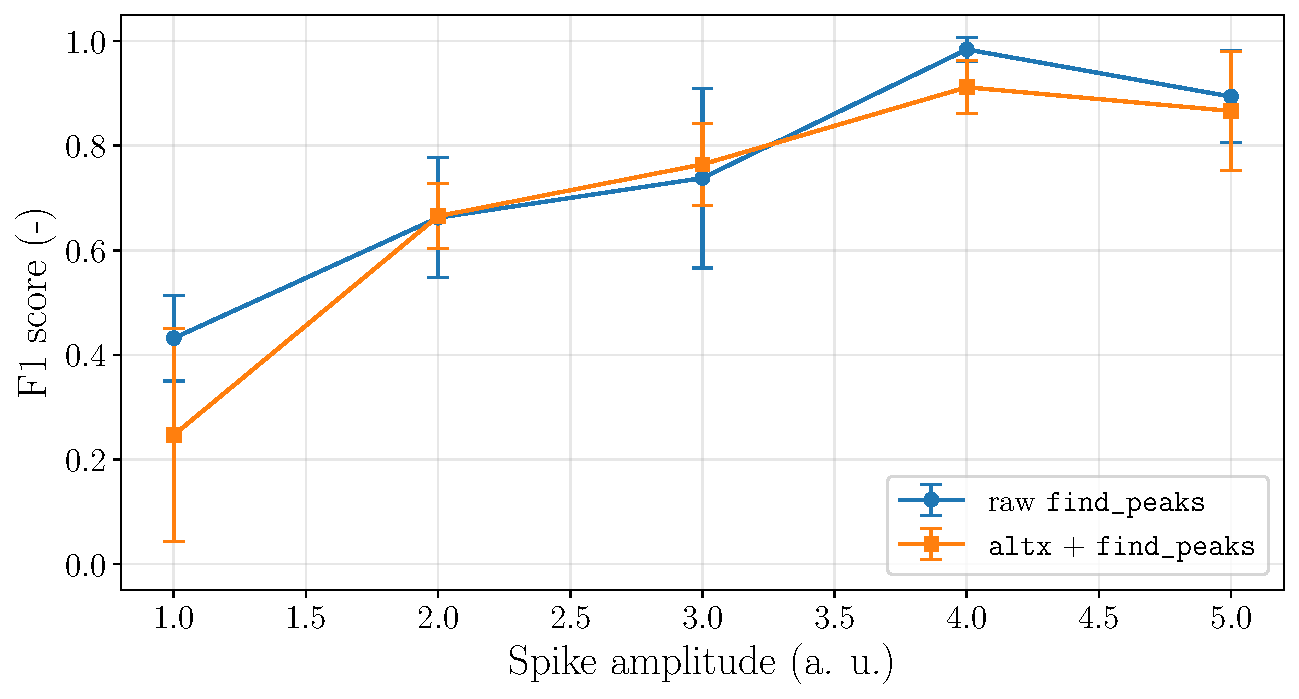
\includegraphics[width=0.66\textwidth]{../img/intro_f1_vs_amplitude.pdf}
  \end{center}
\end{frame}

% ==============================================================
\begin{frame}{What Comes Next}
  Over the coming days we will build this pipeline step by step:
  \begin{itemize}
    \item The mathematics behind the data and the metrics.
    \item Classical signal processing and finding peaks.
    \item The \texttt{altx} method for transforming time series.
    \item Putting it all together into a working anomaly detector.
  \end{itemize}
\end{frame}

\end{document}
